% ============================================================================
%  Payment Platform Simulator — Technical Documentation
%  Compile: pdflatex → bibtex → pdflatex × 2   (or latexmk -pdf)
% ============================================================================
\documentclass[11pt,a4paper,twoside]{article}

% ── Packages ────────────────────────────────────────────────────────────────
\usepackage[utf8]{inputenc}
\usepackage[T1]{fontenc}
\usepackage{lmodern}
\usepackage[margin=2.4cm]{geometry}
\usepackage{graphicx}
\usepackage{xcolor}
\usepackage{hyperref}
\usepackage{listings}
\usepackage{booktabs}
\usepackage{tabularx}
\usepackage{multirow}
\usepackage{enumitem}
\usepackage{tikz}
\usepackage{amsmath}
\usepackage{fancyhdr}
\usepackage{titlesec}
\usepackage{tcolorbox}
\usepackage{float}
\usepackage{caption}
\usepackage{subcaption}
\usepackage{pifont}

\usetikzlibrary{shapes.geometric, arrows.meta, positioning, calc, fit, backgrounds}

% ── Colours ─────────────────────────────────────────────────────────────────
\definecolor{primary}{HTML}{2196F3}
\definecolor{secondary}{HTML}{F50057}
\definecolor{accent}{HTML}{667EEA}
\definecolor{success}{HTML}{4CAF50}
\definecolor{warning}{HTML}{FF9800}
\definecolor{danger}{HTML}{F44336}
\definecolor{codebg}{HTML}{F5F7FA}
\definecolor{codeframe}{HTML}{E0E0E0}
\definecolor{codekw}{HTML}{7C4DFF}
\definecolor{codecomment}{HTML}{9E9E9E}
\definecolor{codestring}{HTML}{43A047}

% ── Hyperref setup ──────────────────────────────────────────────────────────
\hypersetup{
  colorlinks  = true,
  linkcolor   = primary,
  urlcolor    = accent,
  citecolor   = primary,
  pdfauthor   = {Yash Verma},
  pdftitle    = {Payment Platform Simulator — Technical Documentation},
  pdfsubject  = {Enterprise Payment Processing Architecture},
}

% ── Listings ────────────────────────────────────────────────────────────────
\lstdefinestyle{tsStyle}{
  language=Java,
  basicstyle=\ttfamily\small,
  backgroundcolor=\color{codebg},
  frame=single,
  rulecolor=\color{codeframe},
  keywordstyle=\color{codekw}\bfseries,
  commentstyle=\color{codecomment}\itshape,
  stringstyle=\color{codestring},
  showstringspaces=false,
  breaklines=true,
  tabsize=2,
  xleftmargin=4pt,
  xrightmargin=4pt,
  aboveskip=8pt,
  belowskip=8pt,
  morekeywords={async,await,export,interface,enum,const,let,import,from,
                Promise,Map,Set,string,number,boolean,any,void,null,
                undefined,class,extends,implements,private,static,
                readonly,type,Record},
  literate={=>}{{\textcolor{codekw}{=>}}}{2},
  captionpos=b,
}
\lstset{style=tsStyle}

% ── Headers / footers ──────────────────────────────────────────────────────
\pagestyle{fancy}
\fancyhf{}
\fancyhead[LE,RO]{\thepage}
\fancyhead[RE]{\textit{Payment Platform Simulator}}
\fancyhead[LO]{\textit{\nouppercase{\leftmark}}}
\renewcommand{\headrulewidth}{0.4pt}

% ── tcolorbox styles ───────────────────────────────────────────────────────
\tcbuselibrary{skins,breakable}
\newtcolorbox{infobox}[1][]{
  colback=primary!5, colframe=primary!70!black,
  fonttitle=\bfseries, title={#1},
  arc=2mm, breakable
}
\newtcolorbox{warnbox}[1][]{
  colback=warning!8, colframe=warning!70!black,
  fonttitle=\bfseries, title={#1},
  arc=2mm, breakable
}
\newtcolorbox{keyinsight}[1][]{
  colback=accent!6, colframe=accent!70!black,
  fonttitle=\bfseries, title={#1},
  arc=2mm, breakable
}

% ── Section styling ────────────────────────────────────────────────────────
\titleformat{\section}
  {\Large\bfseries\color{primary}}{\thesection}{1em}{}[\vspace{2pt}\titlerule]
\titleformat{\subsection}
  {\large\bfseries\color{primary!80!black}}{\thesubsection}{1em}{}
\titleformat{\subsubsection}
  {\normalsize\bfseries\color{primary!60!black}}{\thesubsubsection}{1em}{}

% ── Shortcuts ──────────────────────────────────────────────────────────────
\newcommand{\cmark}{\ding{51}}
\newcommand{\xmark}{\ding{55}}
\newcommand{\code}[1]{\texttt{\small #1}}

% ============================================================================
%  TITLE PAGE
% ============================================================================
\begin{document}
\begin{titlepage}
\centering
\vspace*{2cm}

{\Huge\bfseries\color{primary} Payment Platform Simulator}\\[0.6cm]
{\Large\color{primary!70!black} Enterprise-Grade Payment Processing Architecture}\\[1.2cm]


\begin{tikzpicture}
  \draw[line width=2pt, accent] (0,0) -- (12,0);
\end{tikzpicture}\\[1.5cm]

{\large\textbf{Technical Documentation \& Architectural Reference}}\\[0.5cm]
{\normalsize Version 1.0 \quad|\quad February 2026}\\[2.5cm]

\begin{tabular}{rl}
  \textbf{Author}      & Yash Verma \\[4pt]
  \textbf{Stack}        & TypeScript\;\textbullet\;Fastify\;\textbullet\;React\;\textbullet\;PostgreSQL \\
                        & Redis\;\textbullet\;RabbitMQ\;\textbullet\;Prisma\;\textbullet\;Docker \\[4pt]
  \textbf{Codebase}     & $\sim$10{,}000 lines \quad|\quad 84 files \quad|\quad 180 tests \\[4pt]
  \textbf{Coverage}     & $\sim$80\% line coverage \\[4pt]
  \textbf{License}      & MIT \\
\end{tabular}

\vfill
{\small\color{gray} This document is generated from the source code and README of the project.}
\end{titlepage}

% ============================================================================
%  TABLE OF CONTENTS
% ============================================================================
\tableofcontents
\newpage

% ============================================================================
\section{Executive Summary}
% ============================================================================

The \textbf{Payment Platform Simulator} is a production-ready, full-stack payment
processing system built as both a \emph{learning resource} for engineers and a
\emph{reference implementation} for scalable fintech architectures. It enables
developers to test payment integrations, simulate failure scenarios, and validate
resilience patterns—\emph{without} connecting to real gateways, incurring
transaction fees, or managing PCI compliance.

\begin{infobox}[Key Metrics]
\begin{tabularx}{\textwidth}{lX}
  \toprule
  \textbf{Metric} & \textbf{Value} \\
  \midrule
  Architecture Patterns  & 8 (Event Sourcing, CQRS, Circuit Breaker, Strategy, Factory, Singleton, Pub/Sub, Middleware) \\
  Test Coverage          & 180 tests across 32 suites ($\sim$80\% line coverage) \\
  Lines of Code          & $\sim$9{,}900 TypeScript across 84 source files \\
  Independent Services   & 13 (Payment, Auth, Gateway×4, 3DS, Circuit Breaker, Event Store, CQRS Query, WebSocket, Webhook, Simulator) \\
  API Endpoints          & 25+ RESTful routes with Swagger/OpenAPI \\
  Database Models        & 17 Prisma models + 9 enums \\
  Real-time Support      & WebSocket (Socket.IO) with topic-based pub/sub \\
  Multi-Gateway          & Stripe, PayPal, Razorpay + Simulator \\
  Security               & JWT rotation + RBAC (5 roles, 10 permissions) + 3D Secure 2.0 \\
  \bottomrule
\end{tabularx}
\end{infobox}

% ============================================================================
\section{Problem Statement \& Motivation}
% ============================================================================

Payment integration in modern applications is deceptively complex. Five primary
challenges drive the need for a dedicated simulator:

\begin{enumerate}[leftmargin=2em]
  \item \textbf{Testing Cost.} Live sandbox accounts still incur fees and offer
        limited edge-case coverage.
  \item \textbf{Edge-Case Simulation.} Timeouts, declines, gateway outages, and
        race conditions are difficult to reproduce deterministically.
  \item \textbf{Compliance \& Security.} PCI DSS, Strong Customer Authentication
        (SCA/3DS), and audit-trail requirements demand specialised tooling.
  \item \textbf{Resilience Validation.} Retry logic, idempotency enforcement, and
        circuit-breaker behaviour need controlled failure injection.
  \item \textbf{Multi-Gateway Portability.} Differing APIs across Stripe, PayPal,
        and Razorpay create vendor lock-in risk.
\end{enumerate}

\begin{keyinsight}[Solution]
A \emph{complete} simulator that provides zero-cost testing via deterministic
test cards, implements production design patterns (event sourcing, CQRS, circuit
breakers), supports multi-gateway failover, and ships with a React dashboard for
real-time observability.
\end{keyinsight}

% ============================================================================
\section{System Architecture}
\label{sec:architecture}
% ============================================================================

\subsection{High-Level Architecture Diagram}

\begin{figure}[H]
\centering
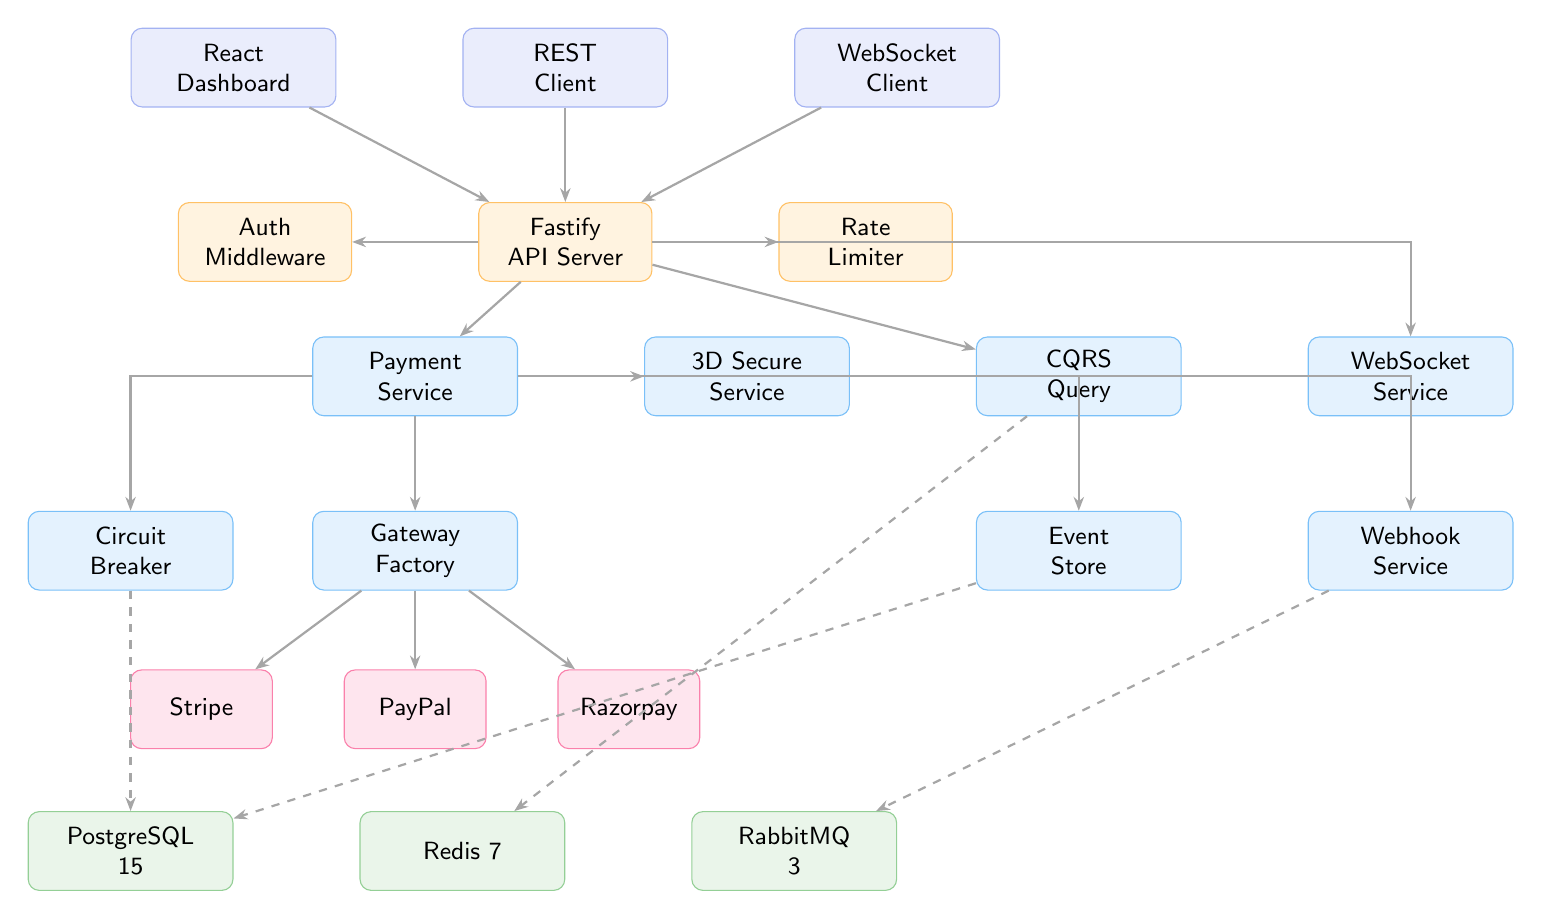
\begin{tikzpicture}[
  node distance=1.0cm and 1.6cm,
  box/.style={draw, rounded corners=4pt, minimum height=1.0cm,
              minimum width=2.6cm, align=center, font=\small\sffamily},
  service/.style={box, fill=primary!12, draw=primary!60},
  infra/.style={box, fill=success!12, draw=success!60},
  client/.style={box, fill=accent!14, draw=accent!60},
  mid/.style={box, fill=warning!12, draw=warning!60, minimum width=2.2cm},
  arr/.style={-{Stealth[length=5pt]}, thick, color=gray!70},
]
  % Clients
  \node[client] (react) {React\\Dashboard};
  \node[client, right=of react] (curl) {REST\\Client};
  \node[client, right=of curl] (ws) {WebSocket\\Client};

  % API Layer
  \node[mid, below=1.2cm of curl] (fastify) {Fastify\\API Server};

  % Middleware
  \node[mid, left=of fastify] (auth) {Auth\\Middleware};
  \node[mid, right=of fastify] (rate) {Rate\\Limiter};

  % Core Services
  \node[service, below=1.2cm of $(auth)!0.5!(fastify)$] (payment) {Payment\\Service};
  \node[service, right=of payment] (threeds) {3D Secure\\Service};
  \node[service, right=of threeds] (cqrs) {CQRS\\Query};

  % Gateway Layer
  \node[service, below=1.2cm of payment] (factory) {Gateway\\Factory};
  \node[service, left=1.0cm of factory] (cb) {Circuit\\Breaker};

  % Adapters
  \node[box, fill=secondary!10, draw=secondary!50, below left=1.0cm and 0.5cm of factory, minimum width=1.8cm] (stripe) {Stripe};
  \node[box, fill=secondary!10, draw=secondary!50, below=1.0cm of factory, minimum width=1.8cm] (paypal) {PayPal};
  \node[box, fill=secondary!10, draw=secondary!50, below right=1.0cm and 0.5cm of factory, minimum width=1.8cm] (razorpay) {Razorpay};

  % Supporting Services
  \node[service, below=1.2cm of cqrs] (events) {Event\\Store};
  \node[service, right=of events] (webhook) {Webhook\\Service};
  \node[service, right=of cqrs] (wsserv) {WebSocket\\Service};

  % Infrastructure
  \node[infra, below=2.8cm of cb] (pg) {PostgreSQL\\15};
  \node[infra, right=of pg] (redis) {Redis 7};
  \node[infra, right=of redis] (rabbit) {RabbitMQ\\3};

  % Arrows ─ Client → API
  \draw[arr] (react) -- (fastify);
  \draw[arr] (curl) -- (fastify);
  \draw[arr] (ws) -- (fastify);

  % API → Middleware
  \draw[arr] (fastify) -- (auth);
  \draw[arr] (fastify) -- (rate);

  % API → Services
  \draw[arr] (fastify) -- (payment);
  \draw[arr] (fastify) -- (cqrs);
  \draw[arr] (fastify) -| (wsserv);

  % Payment flow
  \draw[arr] (payment) -- (factory);
  \draw[arr] (payment) -- (threeds);
  \draw[arr] (payment) -| (cb);
  \draw[arr] (payment) -| (events);
  \draw[arr] (payment) -| (webhook);

  % Factory → Adapters
  \draw[arr] (factory) -- (stripe);
  \draw[arr] (factory) -- (paypal);
  \draw[arr] (factory) -- (razorpay);

  % Services → Infra
  \draw[arr, dashed] (events) -- (pg);
  \draw[arr, dashed] (cqrs) -- (redis);
  \draw[arr, dashed] (webhook) -- (rabbit);
  \draw[arr, dashed] (cb) -- (pg);

\end{tikzpicture}
\caption{High-level system architecture showing client layer, API server,
         core services, gateway adapters, and infrastructure.}
\label{fig:hld}
\end{figure}

\subsection{Technology Stack}

\begin{table}[H]
\centering
\caption{Technology choices and rationale.}
\label{tab:techstack}
\begin{tabularx}{\textwidth}{llX}
  \toprule
  \textbf{Layer} & \textbf{Technology} & \textbf{Rationale} \\
  \midrule
  Runtime        & Node.js 20 LTS       & Non-blocking I/O for payment event processing \\
  Language       & TypeScript 5 (strict) & Type safety across 84 files; \code{tsc --noEmit} in CI \\
  API Framework  & Fastify 4.26          & 2--3$\times$ faster than Express; schema-based validation \\
  ORM            & Prisma 5.8            & Type-safe queries; declarative schema with migrations \\
  Database       & PostgreSQL 15         & ACID transactions for financial data; JSONB for metadata \\
  Cache          & Redis 7               & Idempotency keys, CQRS read cache, session storage \\
  Message Queue  & RabbitMQ 3            & Async webhook delivery, notifications, settlement jobs \\
  Frontend       & React 19 + Vite 7     & MUI components, Recharts, Redux Toolkit, Socket.IO \\
  Containerisation & Docker + Compose    & Multi-stage build; non-root user; health checks \\
  CI/CD          & GitHub Actions        & 3-job pipeline: quality (Node 20/22), frontend, Docker \\
  \bottomrule
\end{tabularx}
\end{table}

% ============================================================================
\section{Design Patterns \& Implementation}
\label{sec:patterns}
% ============================================================================

This project deliberately implements eight enterprise design patterns. Each is
described below with its purpose, implementation location, and key code.

% ────────────────────────────────────────────────────────────────────────────
\subsection{Strategy + Factory Pattern — Multi-Gateway Adapters}

\textbf{Problem:} Each payment gateway (Stripe, PayPal, Razorpay) exposes a
different API. The system must support runtime gateway selection per merchant
without scattering conditional logic.

\textbf{Solution:} A shared \code{PaymentGatewayInterface} (Strategy) and a
\code{PaymentGatewayFactory} (Factory) that loads gateway configurations from the
database at startup and returns the correct adapter at runtime.

\begin{lstlisting}[caption={Gateway interface (\code{gateway.interface.ts}).}]
export interface PaymentGatewayInterface {
  processPayment(request: PaymentRequest): Promise<PaymentResponse>;
  refundPayment(transactionId: string, amount: number): Promise<RefundResponse>;
  capturePayment(transactionId: string, amount: number): Promise<CaptureResponse>;
  getPaymentStatus(transactionId: string): Promise<PaymentStatusResponse>;
  verify3DSecure(data: ThreeDSecureData): Promise<ThreeDSecureResponse>;
}
\end{lstlisting}

Four concrete adapters implement this interface:

\begin{table}[H]
\centering
\caption{Gateway adapter characteristics.}
\begin{tabularx}{\textwidth}{lccX}
  \toprule
  \textbf{Adapter} & \textbf{LOC} & \textbf{ID Format} & \textbf{Notable Behaviour} \\
  \midrule
  Stripe    & 155 & \code{ch\_xxx}  & Full test-card routing, card-network detection \\
  PayPal    & 120 & \code{PAY-xxx}  & OAuth-style statuses, 3DS marked ``not applicable'' \\
  Razorpay  & 130 & \code{pay\_xxx} & INR default currency, RuPay network support \\
  Simulator & 145 & \code{sim\_xxx} & Deterministic + probabilistic dual mode \\
  \bottomrule
\end{tabularx}
\end{table}

\begin{lstlisting}[caption={Factory pattern (\code{gateway.factory.ts}, simplified).}]
export class PaymentGatewayFactory {
  private static gateways: Map<GatewayType, PaymentGatewayInterface>
    = new Map();

  static async initialize(): Promise<void> {
    const configs = await prisma.gatewayConfig.findMany({
      where: { isActive: true },
    });
    for (const cfg of configs) {
      const adapter = this.createGateway(cfg.gateway, cfg.apiKey);
      this.gateways.set(cfg.gateway.toLowerCase(), adapter);
    }
    // Simulator always available as fallback
    if (!this.gateways.has('simulator')) {
      this.gateways.set('simulator', new SimulatorGateway());
    }
  }
}
\end{lstlisting}

% ────────────────────────────────────────────────────────────────────────────
\subsection{CQRS — Command Query Responsibility Segregation}

\textbf{Problem:} Analytics queries (aggregations, time-series) are expensive and
should not compete with payment writes for database connections.

\textbf{Solution:} Two separate service classes:

\begin{itemize}[leftmargin=2em]
  \item \textbf{Command side} — \code{PaymentService} (521 LOC): handles all
        mutations: \code{createPayment}, \code{capturePayment},
        \code{refundPayment}, \code{voidPayment}, \code{complete3DSAuthentication}.
  \item \textbf{Query side} — \code{PaymentQueryService} (383 LOC): handles
        analytics, status distributions, and top-customer queries with a
        cache-aside pattern backed by Redis.
\end{itemize}

\begin{lstlisting}[caption={CQRS query with Redis cache-aside.}]
async getPaymentAnalytics(merchantId, startDate, endDate) {
  const cacheKey = `analytics:${merchantId}:${startDate}:${endDate}`;
  const cached = await getCache(cacheKey);
  if (cached) return cached;

  const [total, successful, failed, volume, avg] = await Promise.all([
    prisma.transaction.count({ where: filters }),
    prisma.transaction.count({ where: { ...filters, status: 'CAPTURED' }}),
    prisma.transaction.count({ where: { ...filters, status: 'FAILED' }}),
    prisma.transaction.aggregate({ _sum: { amount: true }, where: filters }),
    prisma.transaction.aggregate({ _avg: { amount: true }, where: filters }),
  ]);

  await setCache(cacheKey, result, 300); // 5-min TTL
  return result;
}
\end{lstlisting}

% ────────────────────────────────────────────────────────────────────────────
\subsection{Event Sourcing}

\textbf{Problem:} Financial systems require a complete, immutable audit trail of
every state change for compliance and debugging.

\textbf{Solution:} An \code{EventStoreService} (266 LOC) that persists every
domain event to a dedicated \code{event\_store} table with causation and
correlation IDs for distributed tracing.

\begin{table}[H]
\centering
\caption{Domain events captured in the event store.}
\begin{tabularx}{\textwidth}{lX}
  \toprule
  \textbf{Event Type} & \textbf{When Emitted} \\
  \midrule
  \code{PAYMENT\_INITIATED}      & Payment creation begins \\
  \code{PAYMENT\_AUTHORIZED}     & Gateway returns authorisation \\
  \code{PAYMENT\_CAPTURED}       & Funds captured (single-step or after auth) \\
  \code{PAYMENT\_FAILED}         & Gateway declines or error occurs \\
  \code{PAYMENT\_REFUNDED}       & Full or partial refund processed \\
  \code{PAYMENT\_VOIDED}         & Authorisation cancelled before capture \\
  \code{PAYMENT\_3DS\_REQUIRED}  & 3D Secure challenge initiated \\
  \code{PAYMENT\_3DS\_COMPLETED} & 3D Secure verification finished \\
  \code{TRANSACTION\_CREATED}    & Transaction record persisted \\
  \code{TRANSACTION\_UPDATED}    & Status transition recorded \\
  \bottomrule
\end{tabularx}
\end{table}

Key capabilities:
\begin{itemize}[leftmargin=2em]
  \item \textbf{Atomic batch writes} via \code{prisma.\$transaction()} for
        multi-event consistency.
  \item \textbf{Stream replay} using \code{AsyncIterable<DomainEvent>} generators
        for aggregate reconstruction.
  \item \textbf{Snapshot support} to optimise replay of high-event aggregates.
  \item \textbf{Event statistics} for monitoring event volume and types.
\end{itemize}

% ────────────────────────────────────────────────────────────────────────────
\subsection{Circuit Breaker}

\textbf{Problem:} A failing payment gateway should not cascade into system-wide
outages. Continued retries to a down gateway waste resources and increase latency.

\textbf{Solution:} A generic \code{CircuitBreaker} class (229 LOC) with three states,
managed by a \code{CircuitBreakerRegistry} that maintains per-gateway breakers.

\begin{figure}[H]
\centering
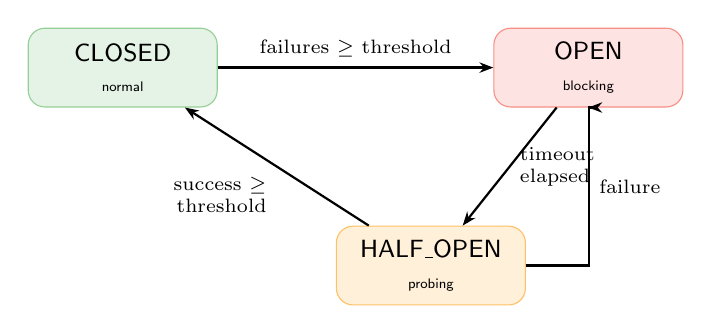
\begin{tikzpicture}[
  state/.style={draw, rounded corners=6pt, minimum width=2.4cm,
                minimum height=1.0cm, align=center, font=\sffamily\small},
  arr/.style={-{Stealth[length=5pt]}, thick},
  node distance=3.5cm,
]
  \node[state, fill=success!15, draw=success!60] (closed) {CLOSED\\{\tiny normal}};
  \node[state, fill=danger!15, draw=danger!60, right=of closed] (open) {OPEN\\{\tiny blocking}};
  \node[state, fill=warning!15, draw=warning!60, below right=1.5cm and 1.5cm of closed] (half) {HALF\_OPEN\\{\tiny probing}};

  \draw[arr] (closed) -- node[above, font=\scriptsize] {failures $\geq$ threshold} (open);
  \draw[arr] (open) -- node[right, font=\scriptsize, align=left] {timeout\\elapsed} (half);
  \draw[arr] (half) -- node[below left, font=\scriptsize, align=right] {success $\geq$\\threshold} (closed);
  \draw[arr] (half.east) -- ++(0.8,0) |- node[near start, right, font=\scriptsize] {failure} (open.south);
\end{tikzpicture}
\caption{Circuit breaker state machine.}
\label{fig:cb}
\end{figure}

\begin{keyinsight}[PostgreSQL-backed state persistence]
Unlike most in-memory circuit breaker implementations, this project persists
breaker state to the \code{circuit\_breaker\_state} table. This means the breaker
survives application restarts and rolling deployments—critical for financial
systems where a ``freshly closed'' breaker could flood a still-recovering gateway.
\end{keyinsight}

\begin{lstlisting}[caption={Circuit breaker wrapping a gateway call.}]
// In PaymentService.createPayment()
const breaker = CircuitBreakerRegistry.getBreaker(`gateway_${gateway}`);
const result = await breaker.execute(async () => {
  return gatewayAdapter.processPayment(paymentRequest);
});
\end{lstlisting}

Configuration defaults:

\begin{table}[H]
\centering
\begin{tabular}{lrl}
  \toprule
  \textbf{Parameter} & \textbf{Default} & \textbf{Description} \\
  \midrule
  \code{failureThreshold}  & 5       & Failures before OPEN \\
  \code{successThreshold}  & 2       & Successes in HALF\_OPEN before CLOSED \\
  \code{timeout}           & 60\,s   & Time in OPEN before probing \\
  \code{monitoringPeriod}  & 120\,s  & Window for failure counting \\
  \bottomrule
\end{tabular}
\end{table}

% ────────────────────────────────────────────────────────────────────────────
\subsection{Idempotency}

\textbf{Problem:} Network retries can cause duplicate payment processing,
resulting in double charges.

\textbf{Solution:} Redis-backed idempotency keys with a 24-hour TTL.

\begin{lstlisting}[caption={Idempotency check in \code{createPayment()}.}]
const idempotencyKey = data.metadata?.idempotencyKey;
if (idempotencyKey) {
  const cached = await getRedis(`idempotency:${idempotencyKey}`);
  if (cached) return JSON.parse(cached); // Return previous result
}

// ... process payment ...

if (idempotencyKey) {
  await setRedis(`idempotency:${idempotencyKey}`, JSON.stringify(result),
                  86400); // 24h TTL
}
\end{lstlisting}

The \code{idempotencyKey} is also stored as a \code{@unique} column on the
\code{Transaction} model, providing database-level deduplication as a second
safety net.

% ────────────────────────────────────────────────────────────────────────────
\subsection{Pub/Sub — WebSocket Real-Time Updates}

\textbf{Problem:} The React dashboard needs immediate feedback when payments
are processed, without polling the API.

\textbf{Solution:} A Singleton \code{WebSocketService} (236 LOC) that manages
client connections with topic-based subscriptions.

\begin{lstlisting}[caption={WebSocket message types.}]
export interface WebSocketMessage {
  type: 'payment_update' | 'transaction_update'
      | 'notification' | 'error';
  data: any;
  timestamp: string;
}
\end{lstlisting}

Each connected client maintains a \code{Set<string>} of subscribed topics.
When a payment is processed, the service broadcasts to all clients subscribed to
the relevant merchant or transaction topic.

% ============================================================================
\section{Payment Lifecycle}
\label{sec:lifecycle}
% ============================================================================

The core \code{createPayment()} method in \code{PaymentService} (521 LOC)
orchestrates \textbf{seven cross-cutting concerns} in a single transactional flow:

\begin{figure}[H]
\centering
\begin{tikzpicture}[
  step/.style={draw, rounded corners=3pt, minimum width=4.5cm,
               minimum height=0.7cm, align=center, font=\small\sffamily,
               fill=primary!8, draw=primary!50},
  arr/.style={-{Stealth[length=4pt]}, thick, color=gray!60},
  node distance=0.5cm,
]
  \node[step] (s1) {1. Idempotency Check (Redis)};
  \node[step, below=of s1] (s2) {2. Validate Payment Method};
  \node[step, below=of s2] (s3) {3. Event: \code{PAYMENT\_INITIATED}};
  \node[step, below=of s3] (s4) {4. Circuit Breaker $\to$ Gateway Adapter};
  \node[step, below=of s4] (s5) {5. 3D Secure Challenge (if required)};
  \node[step, below=of s5] (s6) {6. Persist Transaction + Events};
  \node[step, below=of s6] (s7) {7. WebSocket Broadcast + Webhook Queue};

  \draw[arr] (s1) -- (s2);
  \draw[arr] (s2) -- (s3);
  \draw[arr] (s3) -- (s4);
  \draw[arr] (s4) -- (s5);
  \draw[arr] (s5) -- (s6);
  \draw[arr] (s6) -- (s7);
\end{tikzpicture}
\caption{Payment creation flow — seven orchestrated concerns.}
\label{fig:payment-flow}
\end{figure}

Additional payment operations follow similar patterns:

\begin{table}[H]
\centering
\caption{Payment operations supported.}
\begin{tabularx}{\textwidth}{lX}
  \toprule
  \textbf{Operation} & \textbf{Description} \\
  \midrule
  \code{createPayment()}   & Authorise + optionally capture in a single step \\
  \code{capturePayment()}  & Complete a previously authorised hold \\
  \code{refundPayment()}   & Full or partial refund with amount validation \\
  \code{voidPayment()}     & Cancel authorisation before settlement \\
  \code{complete3DS()}     & Finalise 3D Secure authentication \\
  \code{getPayment()}      & Retrieve payment details by ID \\
  \bottomrule
\end{tabularx}
\end{table}

% ============================================================================
\section{Security Architecture}
\label{sec:security}
% ============================================================================

\subsection{Authentication — Dual System}

The platform supports two authentication mechanisms:

\begin{enumerate}[leftmargin=2em]
  \item \textbf{API Key Authentication} (68 LOC) — For machine-to-machine calls.
        \code{Authorization: Bearer sk\_test\_xxx} header is matched against
        the \code{Merchant.apiKey} column. Suspended merchants are rejected.

  \item \textbf{User Authentication with JWT Rotation} (264 LOC) — For
        human users. Features:
        \begin{itemize}
          \item \textbf{Access tokens:} 15-minute expiry
          \item \textbf{Refresh tokens:} 7-day expiry with automatic rotation
          \item \textbf{Password hashing:} bcrypt with cost factor 12
          \item \textbf{Token revocation:} \code{replacedBy} chain tracking,
                IP/user-agent logging, mass revocation for compromised accounts
          \item \textbf{Cleanup:} Automated expired-token removal
        \end{itemize}
\end{enumerate}

\subsection{Role-Based Access Control (RBAC)}

\begin{table}[H]
\centering
\caption{RBAC roles and their default permissions.}
\begin{tabularx}{\textwidth}{lX}
  \toprule
  \textbf{Role} & \textbf{Default Permissions} \\
  \midrule
  \code{ADMIN}          & Full access (bypasses all permission checks) \\
  \code{MERCHANT\_OWNER}& \code{CREATE\_PAYMENT}, \code{READ\_PAYMENT}, \code{REFUND\_PAYMENT}, \code{MANAGE\_WEBHOOKS}, \code{VIEW\_ANALYTICS} \\
  \code{MERCHANT\_STAFF}& \code{CREATE\_PAYMENT}, \code{READ\_PAYMENT} \\
  \code{CUSTOMER}       & \code{READ\_PAYMENT}, \code{CREATE\_PAYMENT} \\
  \code{API\_USER}      & \code{READ\_PAYMENT}, \code{CREATE\_PAYMENT} \\
  \bottomrule
\end{tabularx}
\end{table}

Two middleware guards enforce access control:
\begin{itemize}[leftmargin=2em]
  \item \code{requirePermission(...perms)} — user must hold \emph{at least one}
        of the listed permissions.
  \item \code{requireRole(...roles)} — user role must match one of the listed roles.
\end{itemize}

\subsection{3D Secure 2.0 Simulation}

The \code{ThreeDSecureService} (317 LOC) simulates a complete EMV 3DS flow:

\begin{enumerate}[leftmargin=2em]
  \item \textbf{Initiation:} Generate authentication request and challenge URL.
  \item \textbf{Challenge:} Create PaReq (Payment Authentication Request,
        base64-encoded).
  \item \textbf{ACS Routing:} Direct to the card network's Authentication Control
        Server URL (Visa, Mastercard, Amex).
  \item \textbf{Verification:} Validate PaRes (Payment Authentication Response).
  \item \textbf{Completion:} Generate ECI, CAVV, and XID values.
\end{enumerate}

Challenges expire after 15 minutes. Card number \code{4000000000006975} forces
3D Secure on every transaction.

\subsection{Additional Security Measures}

\begin{itemize}[leftmargin=2em]
  \item \textbf{Helmet} — HTTP security headers (HSTS, X-Frame-Options, etc.)
  \item \textbf{Rate Limiting} — 1{,}000 requests/minute per IP (configurable)
  \item \textbf{CORS} — Restricted to configured frontend origin
  \item \textbf{PII Redaction} — Card numbers, CVVs, and auth headers
        auto-stripped from all Pino log output:
\end{itemize}

\begin{lstlisting}[caption={Logger with PII redaction.}]
export const logger = pino({
  redact: {
    paths: ['req.headers.authorization',
            '*.card.number', '*.card.cvc', '*.cvv'],
    remove: true,
  },
});
\end{lstlisting}

\begin{itemize}[leftmargin=2em]
  \item \textbf{Webhook Signatures} — Stripe-compatible HMAC-SHA256 with
        timestamp-prefixed payload signing (\code{t=\{ts\},v1=\{sig\}}).
  \item \textbf{Production Secret Validation} — Startup refuses to boot if
        default credentials are detected when \code{NODE\_ENV=production}.
\end{itemize}

% ============================================================================
\section{Data Model}
\label{sec:datamodel}
% ============================================================================

The Prisma schema defines \textbf{17 models} and \textbf{9 enums} in 418 lines.
The entity-relationship overview is shown below.

\begin{table}[H]
\centering
\caption{Core data models and their purpose.}
\begin{tabularx}{\textwidth}{llX}
  \toprule
  \textbf{Model} & \textbf{Key Fields} & \textbf{Purpose} \\
  \midrule
  \code{Merchant}           & apiKey, feeRate, status         & Multi-tenant merchant accounts \\
  \code{User}               & role, permissions, passwordHash & RBAC users with bcrypt auth \\
  \code{RefreshToken}       & token, replacedBy, ipAddress    & JWT rotation chain tracking \\
  \code{Customer}           & email, merchantId               & Per-merchant customer records \\
  \code{PaymentMethod}      & token, last4, brand             & Tokenised card storage \\
  \code{Transaction}        & amount, status, idempotencyKey  & Core financial record \\
  \code{TransactionEvent}   & eventType, previousStatus       & Audit trail per transaction \\
  \code{Settlement}         & grossAmount, netAmount          & Batch settlement aggregation \\
  \code{Webhook}            & url, events[], secret           & Webhook endpoint subscriptions \\
  \code{WebhookDelivery}    & status, retryCount, nextRetryAt & Delivery tracking with retry \\
  \code{SimulatorConfig}    & successRate, delayMs            & Per-merchant simulator tuning \\
  \code{ThreeDSecure}       & eci, cavv, xid, status          & 3DS authentication records \\
  \code{GatewayConfig}      & gateway, apiKey, isPrimary      & Multi-gateway config per merchant \\
  \code{EventStore}         & aggregateId, eventData, version & Event sourcing journal \\
  \code{CircuitBreakerState}& state, failureCount             & Persistent breaker state \\
  \bottomrule
\end{tabularx}
\end{table}

\begin{infobox}[Indexing Strategy]
15+ composite and single-column indices are defined on high-cardinality columns
(\code{merchantId + createdAt}, \code{status}, \code{idempotencyKey},
\code{aggregateId + aggregateType}) to ensure sub-millisecond query performance
even at scale.
\end{infobox}

% ============================================================================
\section{Simulator Engine}
\label{sec:simulator}
% ============================================================================

The simulator operates in two complementary modes:

\subsection{Deterministic Mode — Test Cards}

Ten test card numbers produce \emph{predictable} outcomes, enabling repeatable
integration tests:

\begin{table}[H]
\centering
\caption{Deterministic test card scenarios.}
\begin{tabularx}{\textwidth}{lllX}
  \toprule
  \textbf{Card Number} & \textbf{Network} & \textbf{Result} & \textbf{Description} \\
  \midrule
  4242 4242 4242 4242 & Visa       & \textcolor{success}{\cmark~Success}  & Payment succeeds \\
  5555 5555 5555 4444 & Mastercard & \textcolor{success}{\cmark~Success}  & Payment succeeds \\
  3782 8224 6310 005  & Amex       & \textcolor{success}{\cmark~Success}  & Payment succeeds \\
  4000 0000 0000 0002 & Visa       & \textcolor{danger}{\xmark~Declined}  & Generic card decline \\
  4000 0000 0000 9995 & Visa       & \textcolor{danger}{\xmark~Failed}    & Insufficient funds \\
  4000 0000 0000 0069 & Visa       & \textcolor{danger}{\xmark~Failed}    & Expired card \\
  4000 0000 0000 0127 & Visa       & \textcolor{danger}{\xmark~Failed}    & Incorrect CVC \\
  4000 0000 0000 0341 & Visa       & \textcolor{danger}{\xmark~Failed}    & Processing error \\
  4000 0000 0000 6975 & Visa       & \textcolor{warning}{3DS Required}    & Forces 3D Secure \\
  4000 0000 0000 0259 & Visa       & \textcolor{warning}{Risk Flagged}    & Fraud system flag \\
  \bottomrule
\end{tabularx}
\end{table}

\subsection{Probabilistic Mode — Configurable Failure Distribution}

When a card number does not match a deterministic scenario, the simulator uses a
configurable probability model:

\begin{itemize}[leftmargin=2em]
  \item \textbf{Success rate:} Default 85\%, adjustable 0--100\% via API or UI
  \item \textbf{Failure distribution:} Per-failure-type weights (insufficient
        funds, declined, expired, CVC error, processing error)
  \item \textbf{Network delay:} Configurable min/max latency (default 500--2000\,ms)
  \item \textbf{Fraud detection:} Optional fraud-flagging simulation
\end{itemize}

All parameters are stored in the \code{SimulatorConfig} table and can be
adjusted live via the REST API (\code{PUT /v1/simulator/config}) or the React
dashboard's Simulator page.

% ============================================================================
\section{Frontend Application}
\label{sec:frontend}
% ============================================================================

The React frontend ($\sim$2{,}700 LOC) provides a real-time operational
dashboard built with Material UI, Redux Toolkit, React Query, and Recharts.

\subsection{Pages}

\begin{table}[H]
\centering
\caption{Frontend pages and functionality.}
\begin{tabularx}{\textwidth}{llX}
  \toprule
  \textbf{Page} & \textbf{LOC} & \textbf{Features} \\
  \midrule
  Dashboard    & 285 & Four stat cards (total, successful, failed, revenue); bar chart
                       via Recharts; recent transaction list \\
  Payments     & 374 & Payment creation form with 6 test-card presets; real-time
                       success/error feedback; auto-populated defaults \\
  Transactions & 371 & Filterable transaction table with status chips; refund dialog
                       with amount validation; auto-refresh after refund \\
  Simulator    & 425 & Success rate slider; min/max delay configuration; per-failure-type
                       distribution sliders; 10 test-scenario reference table \\
  \bottomrule
\end{tabularx}
\end{table}

\subsection{Real-Time Architecture}

A custom \code{useWebSocket} hook (129 LOC) connects to the backend Socket.IO
endpoint and:
\begin{itemize}[leftmargin=2em]
  \item Auto-authenticates with the merchant ID on connection
  \item Dispatches Redux actions on \code{payment\_update} and
        \code{transaction\_update} events
  \item Provides \code{subscribe}/\code{unsubscribe} for topic-based channels
  \item Tracks connection state for UI indicators
\end{itemize}

\subsection{State Management}

Redux Toolkit with three slices:
\begin{itemize}[leftmargin=2em]
  \item \code{authSlice} — User login, session management
  \item \code{paymentSlice} — Payment creation state, loading/error tracking
  \item \code{transactionSlice} — Transaction list, filters, real-time updates
\end{itemize}

% ============================================================================
\section{Infrastructure \& DevOps}
\label{sec:infra}
% ============================================================================

\subsection{Docker Setup}

\subsubsection{Multi-Stage Dockerfile}

The production image uses a 4-stage build for minimal size and security:

\begin{table}[H]
\centering
\caption{Docker build stages.}
\begin{tabularx}{\textwidth}{llX}
  \toprule
  \textbf{Stage} & \textbf{Base} & \textbf{Purpose} \\
  \midrule
  \code{base}    & \code{node:20-alpine} & Set working directory \\
  \code{deps}    & \code{base}           & \code{npm ci} — install dependencies only \\
  \code{builder} & \code{deps}           & Prisma generate + TypeScript compile \\
  \code{runner}  & \code{base}           & Production image; non-root user (\code{UID 1001}); copies \code{dist/} only \\
  \bottomrule
\end{tabularx}
\end{table}

\subsubsection{Docker Compose}

Three infrastructure services with health checks and volume persistence:

\begin{table}[H]
\centering
\begin{tabularx}{\textwidth}{lllX}
  \toprule
  \textbf{Service} & \textbf{Image} & \textbf{Port} & \textbf{Health Check} \\
  \midrule
  PostgreSQL & \code{postgres:15-alpine} & 5432 & \code{pg\_isready -U postgres} \\
  Redis      & \code{redis:7-alpine}     & 6379 & \code{redis-cli ping} \\
  RabbitMQ   & \code{rabbitmq:3-mgmt-alpine} & 5672, 15672 & \code{rabbitmq-diagnostics} \\
  \bottomrule
\end{tabularx}
\end{table}

\subsection{CI/CD Pipeline}

GitHub Actions runs a 3-job pipeline on every push to \code{main}/\code{develop}
and on pull requests:

\begin{table}[H]
\centering
\caption{CI pipeline jobs.}
\begin{tabularx}{\textwidth}{llX}
  \toprule
  \textbf{Job} & \textbf{Matrix} & \textbf{Steps} \\
  \midrule
  \code{quality}  & Node 20, 22 & \code{npm ci} $\to$ \code{prisma generate} $\to$ \code{tsc --noEmit} $\to$ lint $\to$ \code{test:coverage} $\to$ upload artifacts \\
  \code{frontend} & Node 20     & \code{npm ci} $\to$ lint $\to$ \code{npm run build} \\
  \code{docker}   & latest      & Docker Buildx $\to$ build image with GHA cache (no push) \\
  \bottomrule
\end{tabularx}
\end{table}

% ============================================================================
\section{Testing Strategy}
\label{sec:testing}
% ============================================================================

\subsection{Overview}

\begin{table}[H]
\centering
\caption{Test suite summary.}
\begin{tabularx}{\textwidth}{lrrX}
  \toprule
  \textbf{Category} & \textbf{Suites} & \textbf{Tests} & \textbf{Framework} \\
  \midrule
  Backend Unit Tests       & 22 & 130 & Jest + ts-jest \\
  Backend Integration Tests & 7 &  35 & Jest + Fastify inject \\
  Frontend Smoke Tests      & 3 &  15 & Vitest + React Testing Library \\
  \midrule
  \textbf{Total}           & \textbf{32} & \textbf{180} & \\
  \bottomrule
\end{tabularx}
\end{table}

\subsection{Coverage Thresholds}

Jest is configured with enforced coverage thresholds in CI:

\begin{table}[H]
\centering
\begin{tabular}{lc}
  \toprule
  \textbf{Metric} & \textbf{Threshold} \\
  \midrule
  Branches   & 70\% \\
  Functions  & 78\% \\
  Lines      & 78\% \\
  Statements & 78\% \\
  \bottomrule
\end{tabular}
\end{table}

\subsection{Test Categories}

\begin{description}[leftmargin=2em, style=nextline]
  \item[Service-Level Unit Tests]
    Each service is tested in isolation with mocked dependencies (Prisma, Redis,
    RabbitMQ). Tests cover happy paths, error handling, edge cases, and boundary
    conditions.

  \item[Middleware Tests]
    Auth middleware (API key lookup, suspended merchant rejection) and RBAC guards
    (permission checks, role validation, admin bypass, token expiry).

  \item[Gateway Adapter Tests]
    Each of the four gateway adapters is tested for: payment processing, decline
    handling, refund flows, capture operations, status checks, and
    3D Secure verification.

  \item[Integration Tests]
    Full HTTP request/response cycles using Fastify's \code{inject()} method.
    Cover all seven route modules: health, payments, merchants, customers,
    transactions, webhooks, and simulator.

  \item[Frontend Smoke Tests]
    Component rendering tests using React Testing Library with JSDOM. Cover the
    Layout (navigation), Dashboard (loading/data/error states), and Payments
    (form fields, test card selection, submit flow).
\end{description}

% ============================================================================
\section{API Reference}
\label{sec:api}
% ============================================================================

Full interactive documentation is available at \code{/docs} (Swagger UI) when
the server is running. Below is a summary of endpoint groups:

\begin{table}[H]
\centering
\caption{API endpoint groups.}
\begin{tabularx}{\textwidth}{llX}
  \toprule
  \textbf{Group} & \textbf{Endpoints} & \textbf{Key Operations} \\
  \midrule
  Health       & 2 & Basic \& detailed health checks \\
  Payments     & 5 & Create, get, capture, refund, void \\
  Merchants    & 2 & Register, get profile \\
  Customers    & 3 & Create, get, list \\
  Transactions & 2 & List (with filters), get by ID \\
  Webhooks     & 3 & Create, list, delete \\
  Simulator    & 3 & Get config, update config, list scenarios \\
  \midrule
  \textbf{Total} & \textbf{20+} & \\
  \bottomrule
\end{tabularx}
\end{table}

\subsection{Example — Create Payment}

\begin{lstlisting}[caption={Create payment request.}]
POST /v1/payments
Authorization: Bearer sk_test_428dbd6d...

{
  "amount": 1000,
  "currency": "usd",
  "payment_method": {
    "type": "card",
    "card": {
      "number": "4242424242424242",
      "exp_month": 12,
      "exp_year": 2027,
      "cvc": "123"
    },
    "billing_details": {
      "name": "Test User",
      "email": "test@example.com"
    }
  },
  "description": "Test payment",
  "capture": true
}
\end{lstlisting}

% ============================================================================
\section{Differentiation from Similar Projects}
\label{sec:differentiation}
% ============================================================================

\begin{table}[H]
\centering
\caption{Feature comparison with typical open-source payment simulators.}
\begin{tabularx}{\textwidth}{Xcc}
  \toprule
  \textbf{Capability} & \textbf{Typical Repos} & \textbf{This Project} \\
  \midrule
  Gateway support                & 1 mock           & 4 adapters (Strategy) \\
  Error simulation               & Random           & 10 deterministic cards \\
  Data persistence               & In-memory / SQLite & PostgreSQL + Redis + RabbitMQ \\
  Real-time updates              & None             & WebSocket (Socket.IO) \\
  Event history                  & Basic logging    & Event sourcing + snapshots \\
  Frontend dashboard             & None / basic     & React + MUI + Charts \\
  Resilience patterns            & None             & Circuit breaker + idempotency \\
  Authentication                 & API key only     & JWT rotation + RBAC + 3DS \\
  CI/CD                          & None             & GitHub Actions (3 jobs) \\
  Documentation                  & README only      & Architecture doc + ADRs + Swagger \\
  Test coverage                  & $<$20\%          & $\sim$80\% (180 tests) \\
  Docker production image        & None / basic     & Multi-stage, non-root user \\
  \bottomrule
\end{tabularx}
\end{table}

% ============================================================================
\section{Project Metrics}
\label{sec:metrics}
% ============================================================================

\begin{table}[H]
\centering
\caption{Codebase metrics (as of February 2026).}
\begin{tabularx}{\textwidth}{Xr}
  \toprule
  \textbf{Metric} & \textbf{Value} \\
  \midrule
  Total TypeScript LOC                    & 9{,}911 \\
  Backend source (\code{src/})            & 4{,}087 \\
  Frontend source (\code{frontend/src/})  & 2{,}718 \\
  Test code (\code{tests/})               & 2{,}988 \\
  Prisma schema + seed                    & 478 \\
  Source files                            & 84 \\
  Prisma models                           & 17 \\
  Prisma enums                            & 9 \\
  Database indices                        & 15+ \\
  REST API endpoints                      & 25+ \\
  Design patterns implemented             & 8 \\
  Test suites                             & 32 \\
  Individual tests                        & 180 \\
  Line coverage                           & $\sim$80\% \\
  npm dependencies (backend)              & 25 \\
  npm dependencies (frontend)             & 18 \\
  Docker build stages                     & 4 \\
  CI pipeline jobs                        & 3 \\
  \bottomrule
\end{tabularx}
\end{table}

% ============================================================================
\section{Getting Started}
\label{sec:quickstart}
% ============================================================================

\subsection{Prerequisites}

\begin{itemize}[leftmargin=2em]
  \item Node.js $\geq$ 20.0.0
  \item Docker \& Docker Compose
  \item Git
\end{itemize}

\subsection{Setup}

\begin{lstlisting}[language=bash, caption={Quick start commands.}]
# Clone and install
git clone https://github.com/yashvyas95/Payment_Platform_Simulator.git
cd Payment_Platform_Simulator
npm install
cd frontend && npm install && cd ..

# Start infrastructure
docker-compose up -d

# Setup database
npx prisma generate
npx prisma migrate deploy
npx prisma db seed

# Start backend (port 3000)
npm run dev

# Start frontend (port 3001) — in a separate terminal
cd frontend && npm run dev
\end{lstlisting}

\subsection{Available URLs}

\begin{table}[H]
\centering
\begin{tabular}{ll}
  \toprule
  \textbf{Service} & \textbf{URL} \\
  \midrule
  Backend API       & \url{http://localhost:3000} \\
  Swagger UI        & \url{http://localhost:3000/docs} \\
  React Dashboard   & \url{http://localhost:3001} \\
  RabbitMQ Console  & \url{http://localhost:15672} \\
  Prisma Studio     & \code{npx prisma studio} (port 5555) \\
  \bottomrule
\end{tabular}
\end{table}

% ============================================================================
\section{Future Roadmap}
\label{sec:roadmap}
% ============================================================================

\begin{enumerate}[leftmargin=2em]
  \item \textbf{Webhook delivery worker} — Consume RabbitMQ queue for async delivery with exponential back-off.
  \item \textbf{Settlement batch processing} — End-of-day aggregation with reconciliation reports.
  \item \textbf{Advanced fraud rules} — Velocity checks, amount thresholds, device fingerprinting.
  \item \textbf{Multi-currency exchange} — Live exchange rates with margin configuration.
  \item \textbf{Load testing suite} — k6 or Artillery scripts for throughput benchmarking.
  \item \textbf{Monitoring stack} — Prometheus metrics + Grafana dashboards.
  \item \textbf{End-to-end tests} — Playwright tests for the full React application.
  \item \textbf{Push coverage to 90\%+} — Target remaining uncovered branches.
\end{enumerate}

% ============================================================================
\section{Conclusion}
% ============================================================================

The Payment Platform Simulator demonstrates that a portfolio project can go
beyond CRUD applications to showcase genuine systems-engineering skills. By
implementing production patterns—event sourcing, CQRS, circuit breakers,
multi-gateway adapters, and comprehensive security—within a cohesive,
well-tested, and containerised application, this project serves as both a
practical learning resource and a credible indicator of enterprise development
capability.

\vspace{1em}
\begin{center}

\begin{tikzpicture}
  \draw[line width=2pt, accent] (0,0) -- (10,0);
\end{tikzpicture}\\[0.5cm]
{\large\color{primary}\textbf{Thank you for reviewing this project.}}\\[0.3cm]
{\small Contributions, feedback, and questions are welcome.}\\[0.2cm]
{\small\url{https://github.com/yashvyas95/Payment_Platform_Simulator}}
\end{center}

\end{document}
